\documentclass{article}

    \usepackage{graphicx}
    \usepackage{indentfirst}
    \usepackage{geometry}
        \geometry{
        a4paper,
        total={170mm,257mm},
        left=20mm,
        top=20mm,
        } 
    \usepackage{hyperref}
    % \hypersetup{
    %         colorlinks=true,
    %         linkcolor=blue,
    %         filecolor=magenta,      
    %         urlcolor=cyan,
    % }
    \newcommand {\weblink}[1]{\href{#1}{\textbf{#1}}}
    \renewcommand{\labelitemi}{$\diamond$}
    \title{CS6630 Project Proposal \protect\\ Visualization for Taxi Rides in New York City}
    \author{Zheng Wang, Yishuai Du}
    \date{October 26, 2018}

\begin{document}
        \maketitle

        \section{Basic Information}
        \begin{itemize} 
           \item Project Title: \textbf{\textit{Visualization for Taxi Rides in New York City}}
           \item Group Members:
           \begin{itemize}
               \item \textbf{Zheng Wang}, u1208847, u1208847@utah.edu
               \item \textbf{Yi Shuai}, u0884588, u0884588@utah.edu 
           \end{itemize}
           \item Project Github Link: \weblink{https://github.com/GregDobby/CS6630VisProj.git}
        \end{itemize}   

        \section{Background and Motivation}

            Dating back to 1605, the horse-drawn hackney carriages can be the first form of taxi. With the development of
            technologies, horse-powered taxis were replaced by electric-powered taxis which were also quickly superseded by gas-powered
            taxis in 1899 in Paris. The advent of the first gas-powered taxi in New York City in 1907 laid the foundation of the largest
            taxi market in the United States. Since then, the taxi industry has become a critical component of the transportation infrastructure
            in large urban areas. Over 800 million consumers are transported annually in the United States, generating \$23 billion revenues.
            
            However, the attention to taxi market regulation was scant until the first momentum of taxi industry in late 1920s, during which price war 
            between taxi companies built threats to the society stability. Unfortunately, similar situtaion seems to happen again these days. 
            Ride-sharing companies, namely Uber and Lyft, offer consumers rides with a lower price and less waiting time, while the incumbent and 
            established taxi companies remain basically the same. And the established companies are doing everything possible to get regulators to help them by
            stopping new entry into their market. The increasingly tense situtaion requires regulation on ride-sharing cars as well as, more importantly,
            exploring more efficient regualtion in taxi industry.

            New entry into taxi market is only an external trigger to alteration of old-fashioned regulation. In fact, the demand for a more efficient regulation
            has always existed as a consequence of inherent characteristics of taxi industry: highly fragmented service, fixed two-part tariff fare regulation 
            and spatial misallocation. A large number of small taxi companies, sometimes of a single owner-operator, result in highly fragmented taxi service. Many
            non-owner taxi drivers who lease cars from taxi companies has to pay a fixed leasing cost and their own gas and insurance. Since the fixed fare rate regulated
            by local municipalities, drivers have to increase their chances to get more consumers to increase their income, which indirectly causes spatial misallocation:
            densely populated area like downtown tends to be over-supplied and sparsely populated area like suburban district tends to be undersupplied. 

            Our project tends to provide a visualizaiton of taxi rides (as well as some sharing rides) in New York City as a useful tool to analyse the relationship between
            supply and demand for a specific period in taxi market and help people adjust the regulation. More specifically, the distribution of people in New York City can vary
            according time in one day, date(weekday, weekend and festivals), weather and some other factors, so the demand can always change. By predicting the demand and adjusting
            the supply and change fare regulation, it can both reduce consumers' waiting time and increase the total revenues, which is a win-win situtaion.  

        \section{Project Objective}
            As the largest taxi industry, there are lots of  taxis compete for consumers by driving to different locations around the New York city. Due to  price regulation and search frictions,  leaving empty taxis in some areas, and leaving excess demand in other areas as a big problem. The spatial mismatch and the waiting time of taxi make reduce lots of daily income. So in our project, we will use a dynamic model of search and matching between taxis and consumers under regulation to optimize this problem.
            In this project, we will show:
            \begin{itemize}
                \item A comparesion between before and after optimization
                \item Map of Estimated Supply and Demand
                \item Taxi Trips and Revenues by Area
                \item Taxi Trip and Fare Summary Statistics
                \item Taxi waiting time at different llocation
                \item consumers waiting time at different location
            \end{itemize}
            
        \section{Data}
            Data visualized are as follows: 
            \begin{itemize}
                \item TLC Trip Record Data in New York City: \\
                    \weblink{http://www.nyc.gov/html/tlc/html/about/trip\_record\_data.shtml}
                \item 2014-2015 Uber Rides in New York City: \\ 
                    \weblink{https://www.kaggle.com/fivethirtyeight/uber-pickups-in-new-york-city}
                \item NYC Zoning GIS Data: \\ 
                    \weblink{https://data.cityofnewyork.us/City-Government/Zoning-GIS-Data-Shapefile/kdig-pewd}
            \end{itemize}
        \section{Data Processing}
            \subsection{TLC Trip Record Data in New York City}
            TLC Trip Record Data in New York City provides us with information about taxi rides in New York City. More specifically, it provides pick up time, 
            drop off time, transportation fare, pick up location and destination. However, to do a useful visualizaiton, we also need demand information such as
            consumers' waiting time and supply information such as taixs' waiting time and cruising area. We will use estimated the data accoding to information provided.

                \begin{enumerate}
                    \item Filter out anomaly values and unnecessary columns such as \textit{store\_and\_fwd\_flag}
                    \item Estimate the number of active taxis by couting different taxis in sampled periods
                    \item Estimate taixs' searching time and consumers' wating time
                    \item Calculate average trip time and transportation fare from a certain zone to another in different periods
                \end{enumerate}
            \subsection{2014-2015 Uber Rides in New York City}
                Data processing for Uber Rides is almost same with TLC Trip Record Data with differences as follows:
                \begin{enumerate}
                    \item Calculate the exact consumers' wating time
                    \item Calculate the exact demand in a specific zone during a certain period
                \end{enumerate}
            \subsection{NYC Zoning GIS Data}
                We use the geojson of New York City without any modification.
        \section{Visualization Design}
                The visualization is divided into two parts. 
                
                \begin{enumerate}
                    \item   \textbf{Map:} The basic unit of the New York City map is \textit{zone} indexed by zone id. For each zone, we will use the color channel
                            to quantify consumers' demand and taxi drivers' supply respectively. Also, a hovering tooltip will display detailed information to support the visulation.
                            By clicking zones on the map, we can set start locations and stop locations to estimate the trip time, which also forms connections between different zones.
                            According to connections between different zones, we can also make comparisons with regard to their basic information such as expected supply, actual supply,
                            supply trend and so on, which can be utilized to adjust taxi regualtion. Moreover, to make a user-friendly interface, we can also do pan, zoom in, zoom out on the map. 
                    \item   \textbf{Sidebar:} The sidebar is further divided into different panels.
                            \begin{itemize}
                                \item Filter Panel: We will implement serveral filters in the filter panel including  time filter, area filter, taxi type filter.
                                \item Chart Panel: Based on applied fiters and connections between selected zones, several statistical charts will be displayed. Biscally,
                                      we will show the demand and supply trend including actual trend and expected trend in selected zones at different time points. Comparisons will also be made
                                      between different zones. What's more, an optional chart will be displayed to illustrate changes after new entry(Uber) entered the taxi market.
                            \end{itemize}
                \end{enumerate}
        \section{Must Have Features}
        \subsection{Side Bar}
        We will have a side bar that contains filter panel and  chart panel.
            
            First, in filter panel we have three sub-features, Date-Time Range feature, Origin and destination zones, and Type.  
            Date-Time Range feature that we can choose the range of date time to get the corresponding data, Origin and destination zones 
            that we can choose the zone of origin and the zone of destination to get the corresponding data base on the datetime you choose. 
            About Type, we will have yellow taxi, green taxi and Uber. In fact,  green taxi and Uber we are consider optional.
            \begin{itemize}
                \item Date-Time Range filter
                \item Origin and destionation zones filter
                \item Type filter
            \end{itemize}

            Second, in charts panel, we will have some statistical charts show some features, such as Taxi Trips and Revenues by Area, 
            Taxi Trip and Fare Summary Statistics, Taxi waiting time at different location, consumers waiting time at different location, average travel time by day and so on.
            \begin{itemize}
                \item Barcharts for revenues, Taxi Trip and Fare Summary Statistics
                \item Linecharts for time trend including Taxi waiting time at different location, consumers waiting time at different location, average travel time by day
            \end{itemize}
        \subsection{Map}

        We will have a geo map contains taxi supply,  consumer demand, and color bar. It is similar to the following:
            The final appearance should be:
            The initial image will show the taxi supply in each zone base on the filter Features in sidebar. We will show each zone as different value with a blue color.
            We will have click button with consumer demand, then the geo map will show each zone as different value with a red color.
            When two zone are select, it will show a connected line and an information bar, to show some statistical value, such as average travel time, average payment, average travel distance, base on the filter Features in sidebar
            When one zone are select, it will show an information bar, to show the average waiting of consumer and taxi base on the filter Features in sidebar
            \begin{itemize}
                \item Visualization for geo data of New York City including pan, zoom operations
                \item Heat map to indicate supply and demand in different zones
                \item Hover tooltips
                \item Click operation to build connections between different zones
            \end{itemize}
 
        \section{Optional Features}
        \begin{itemize}
            \item We will use more types such as Green taxi and Uber to have a comparison.
            \item We will add some dynamic effects if we can get real-time data.
        \end{itemize}
        

        \section{Project Schedule}
            \begin{tabular}{cc}
                \hline
                Week & Assignment \\ \hline
                1& Clean up data and extract features \\
                2& Build frame of the visualization \\
                3& Implement must-have features \\
                4& Finish must-have features and try to implement optional features \\
                5& Review and record a video \\
                \hline

            \end{tabular}
        
        \section{Sketches}
            Project sketches are as follows.

            \begin{figure}[h!]
              \centering
              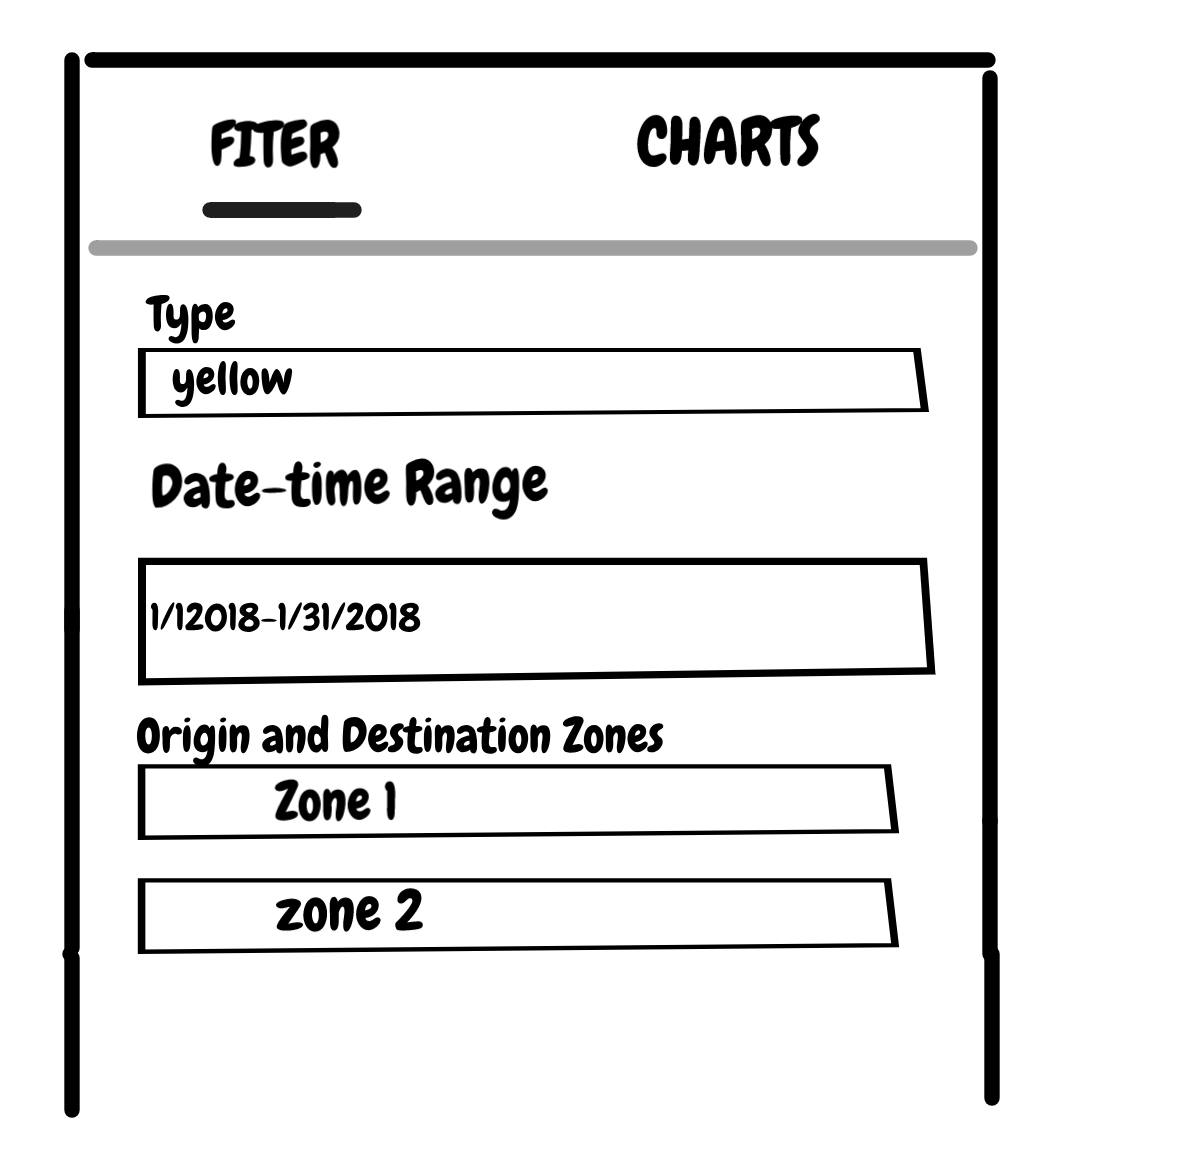
\includegraphics[width=0.5\textwidth]{sketch/filter.png}
              \caption{Filter Panel}
            \end{figure}   
            
            \begin{figure}[h!]
                \centering
                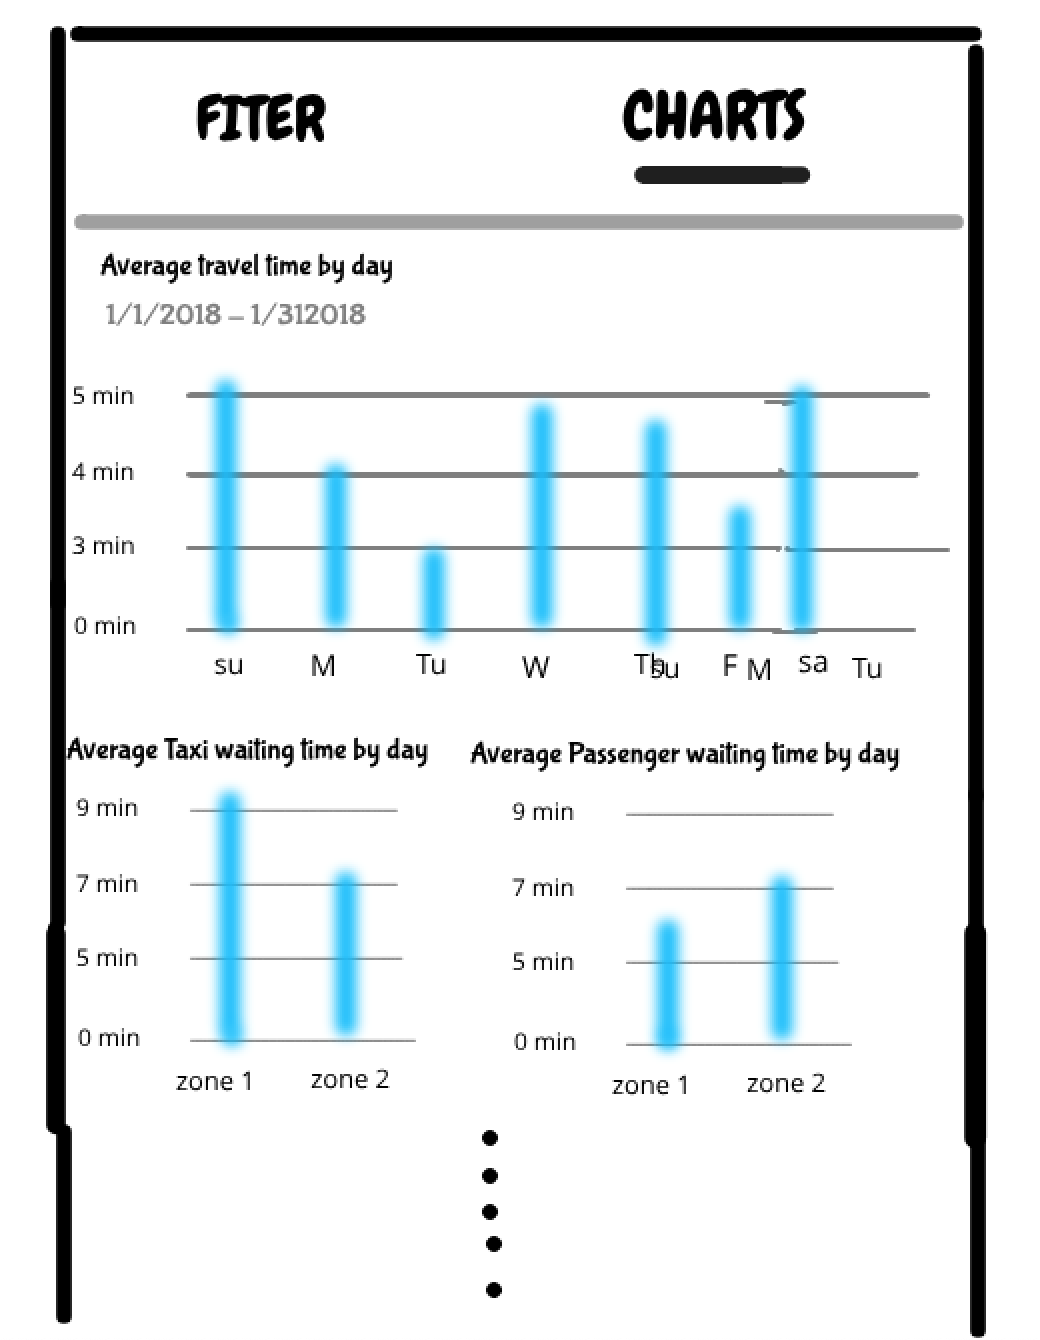
\includegraphics[width=0.5\textwidth]{sketch/chart.png}
                \caption{Chart Panel}
              \end{figure}  
            
              \begin{figure}[h!]
                \centering
                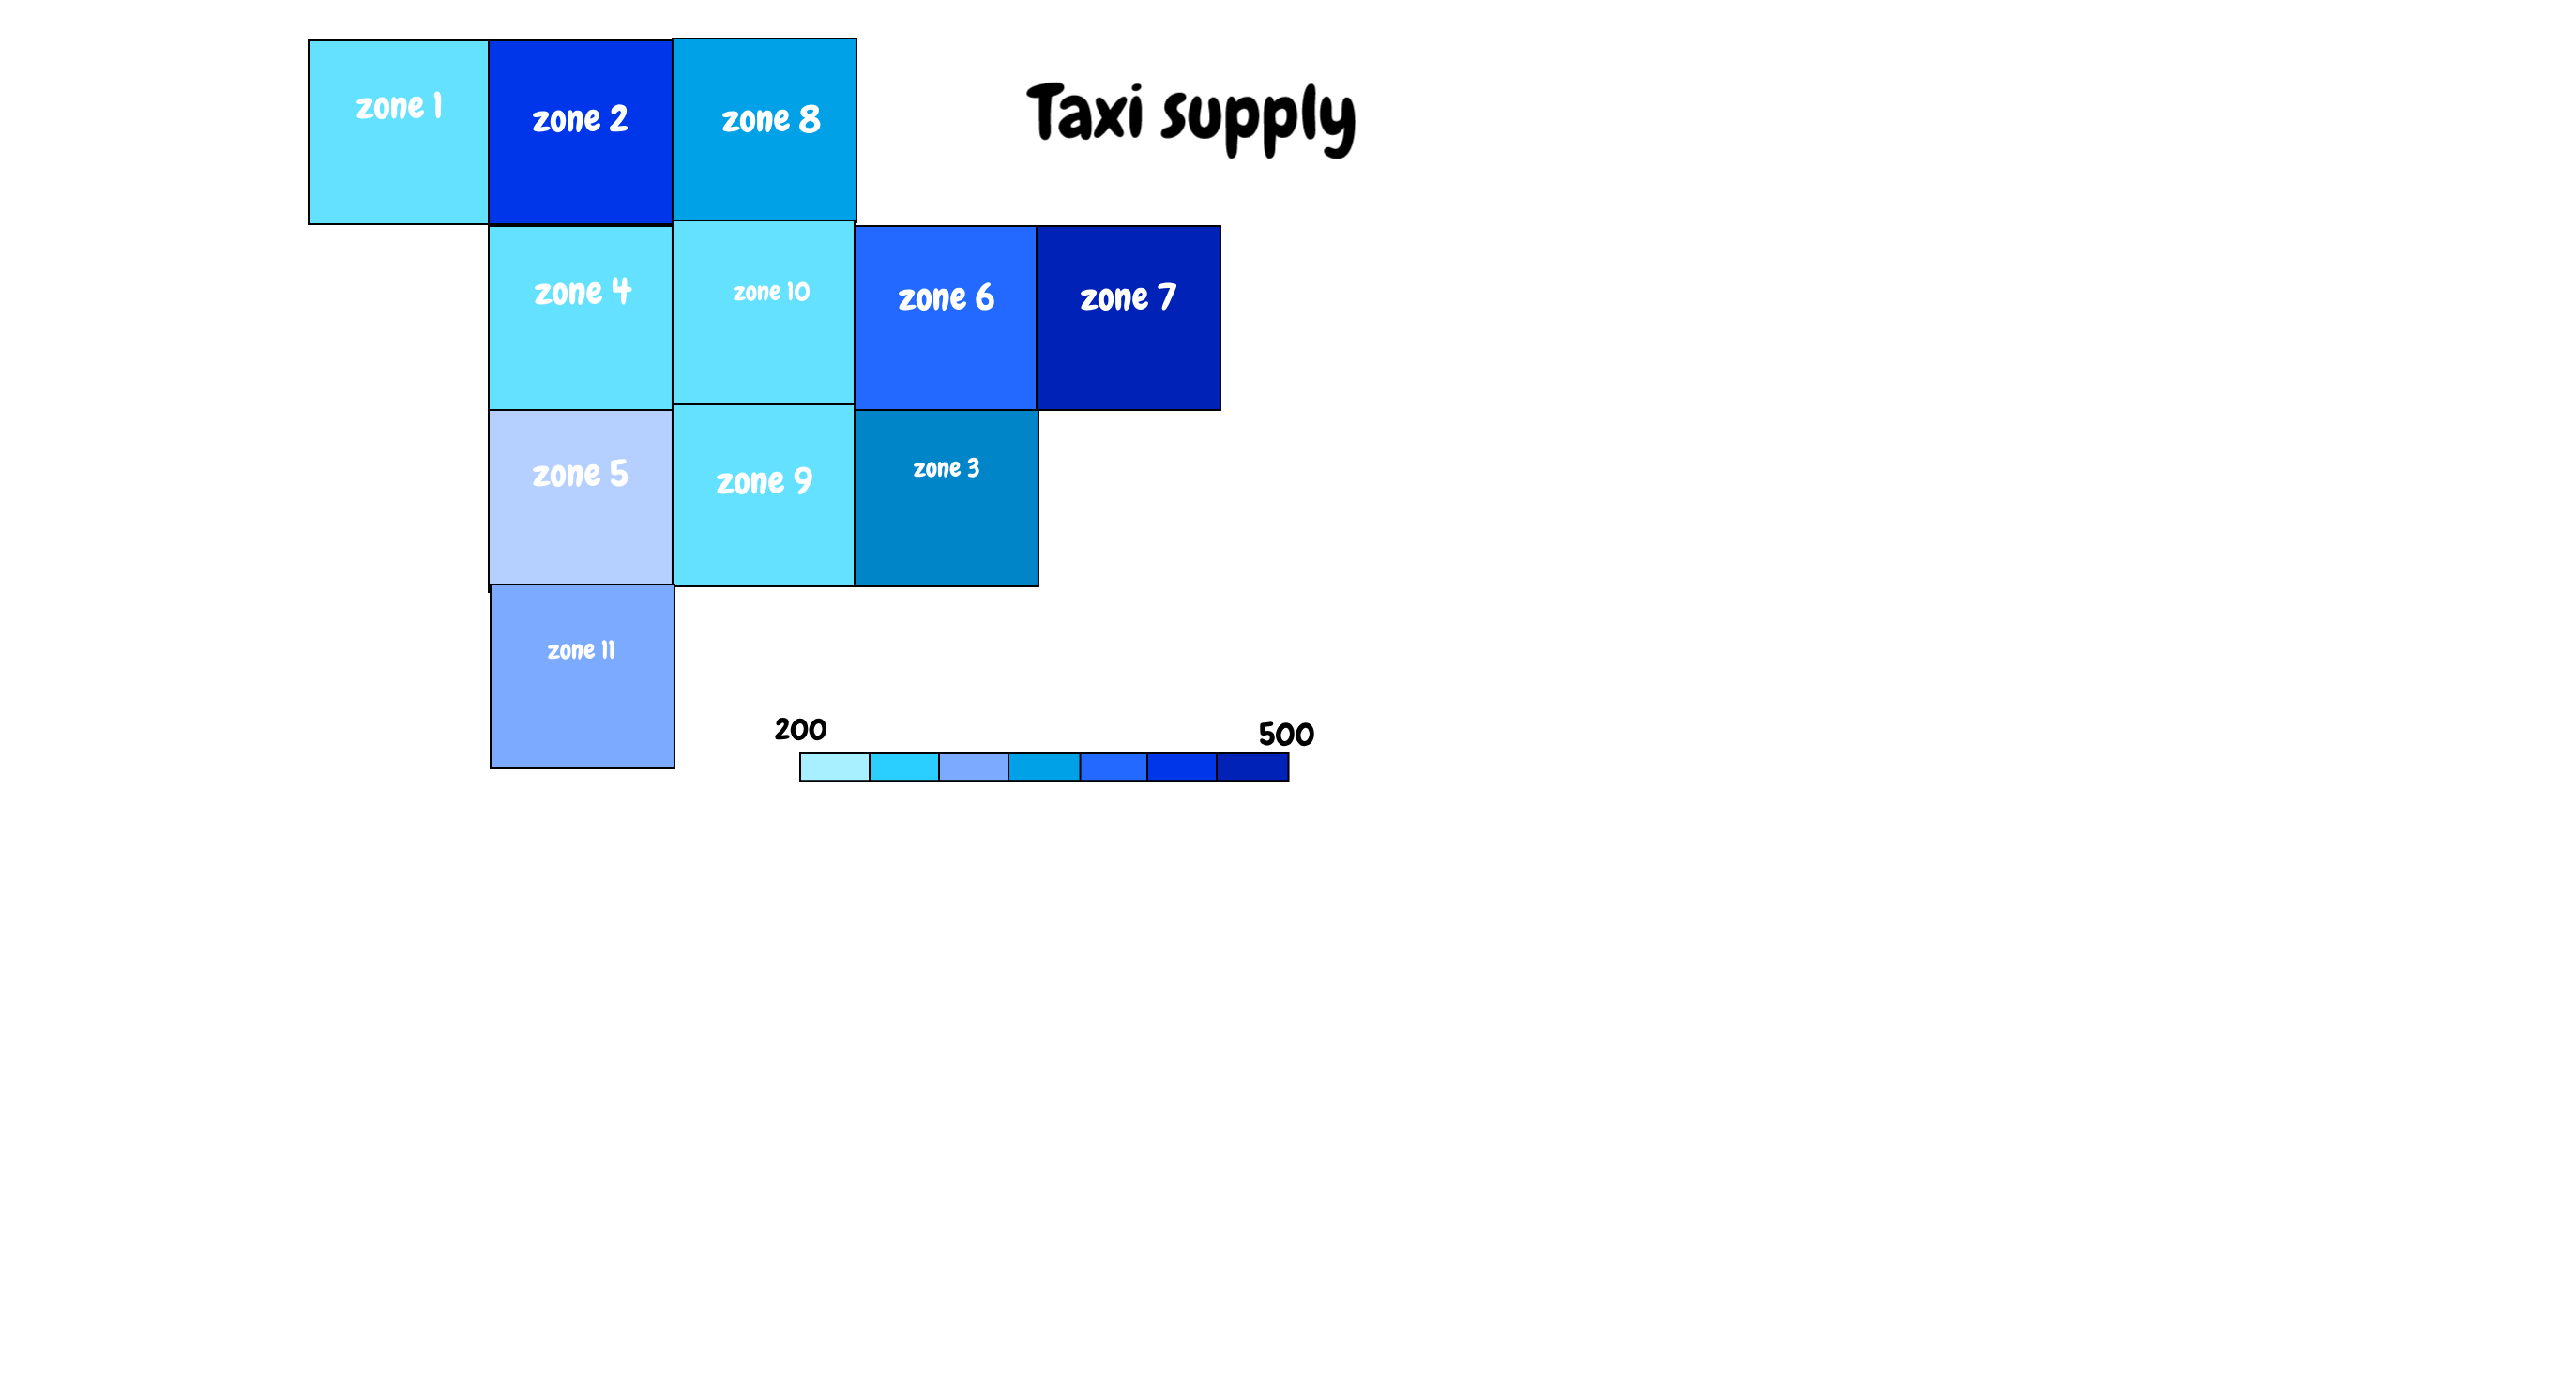
\includegraphics[width=0.8\textwidth]{sketch/taxi_supply.png}
                \caption{Taxi Supply}
              \end{figure} 
              
              \begin{figure}[h!]
                \centering
                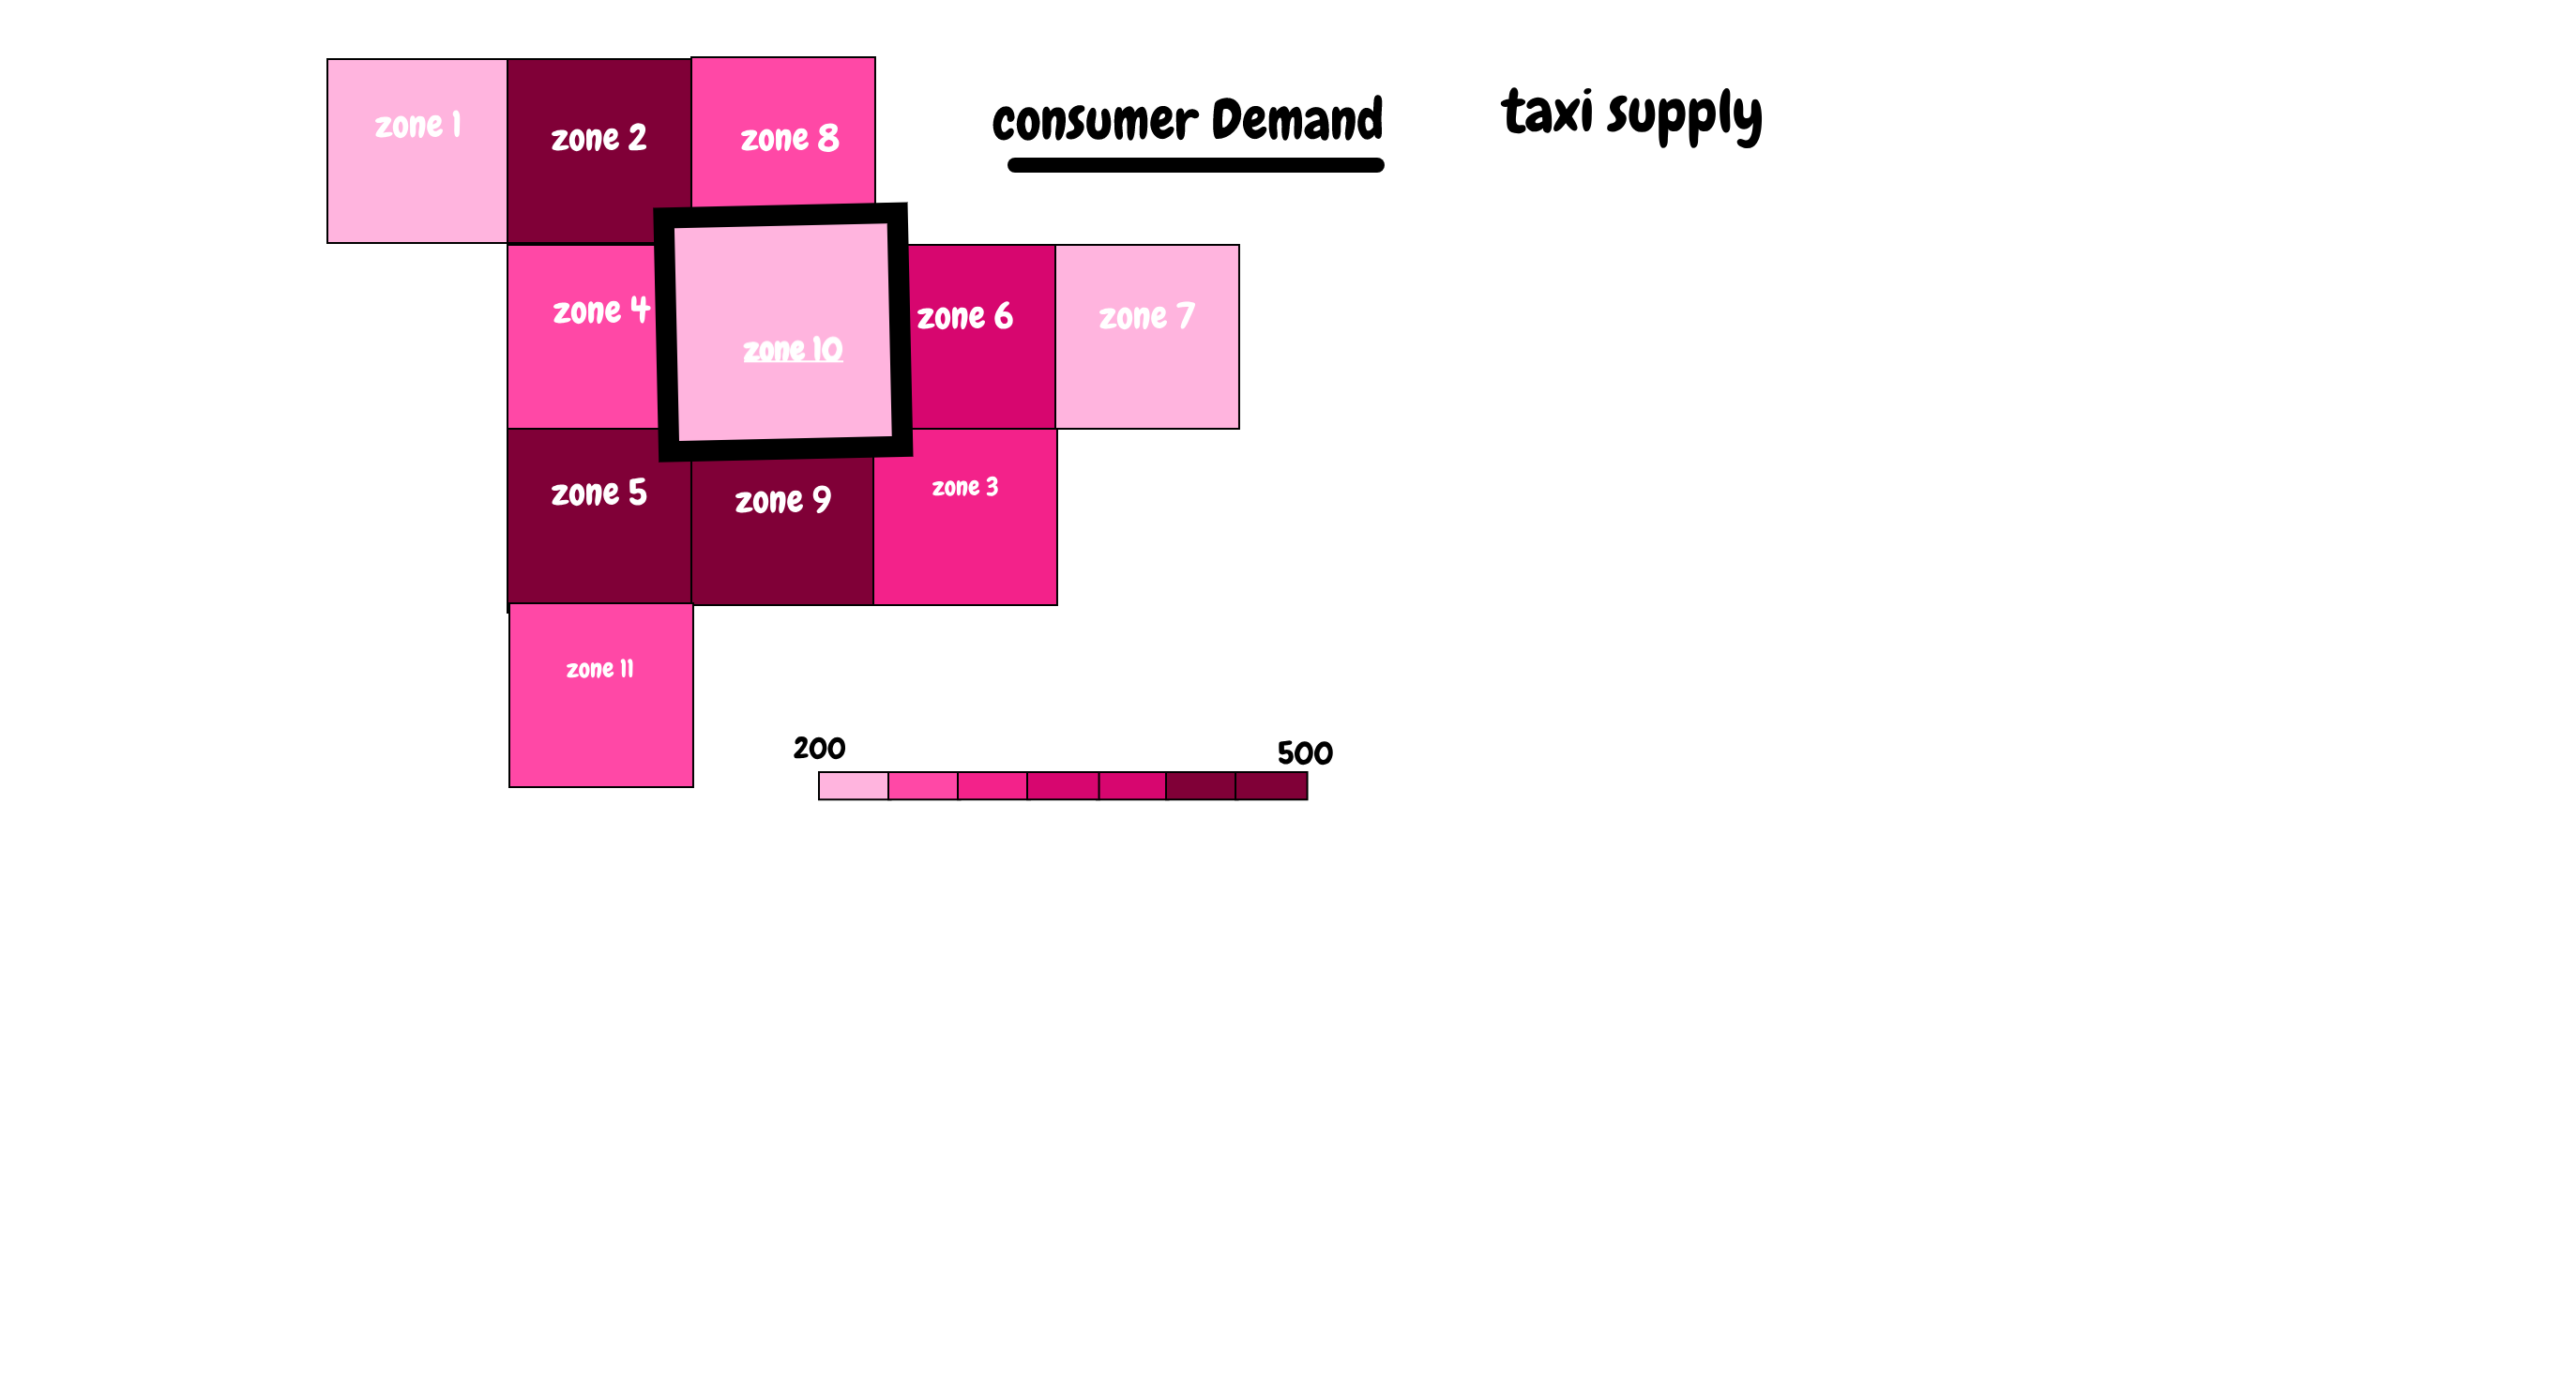
\includegraphics[width=0.8\textwidth]{sketch/consumer_demand.png}
                \caption{Consumer Demand}
              \end{figure}  

              \begin{figure}[h!]
                \centering
                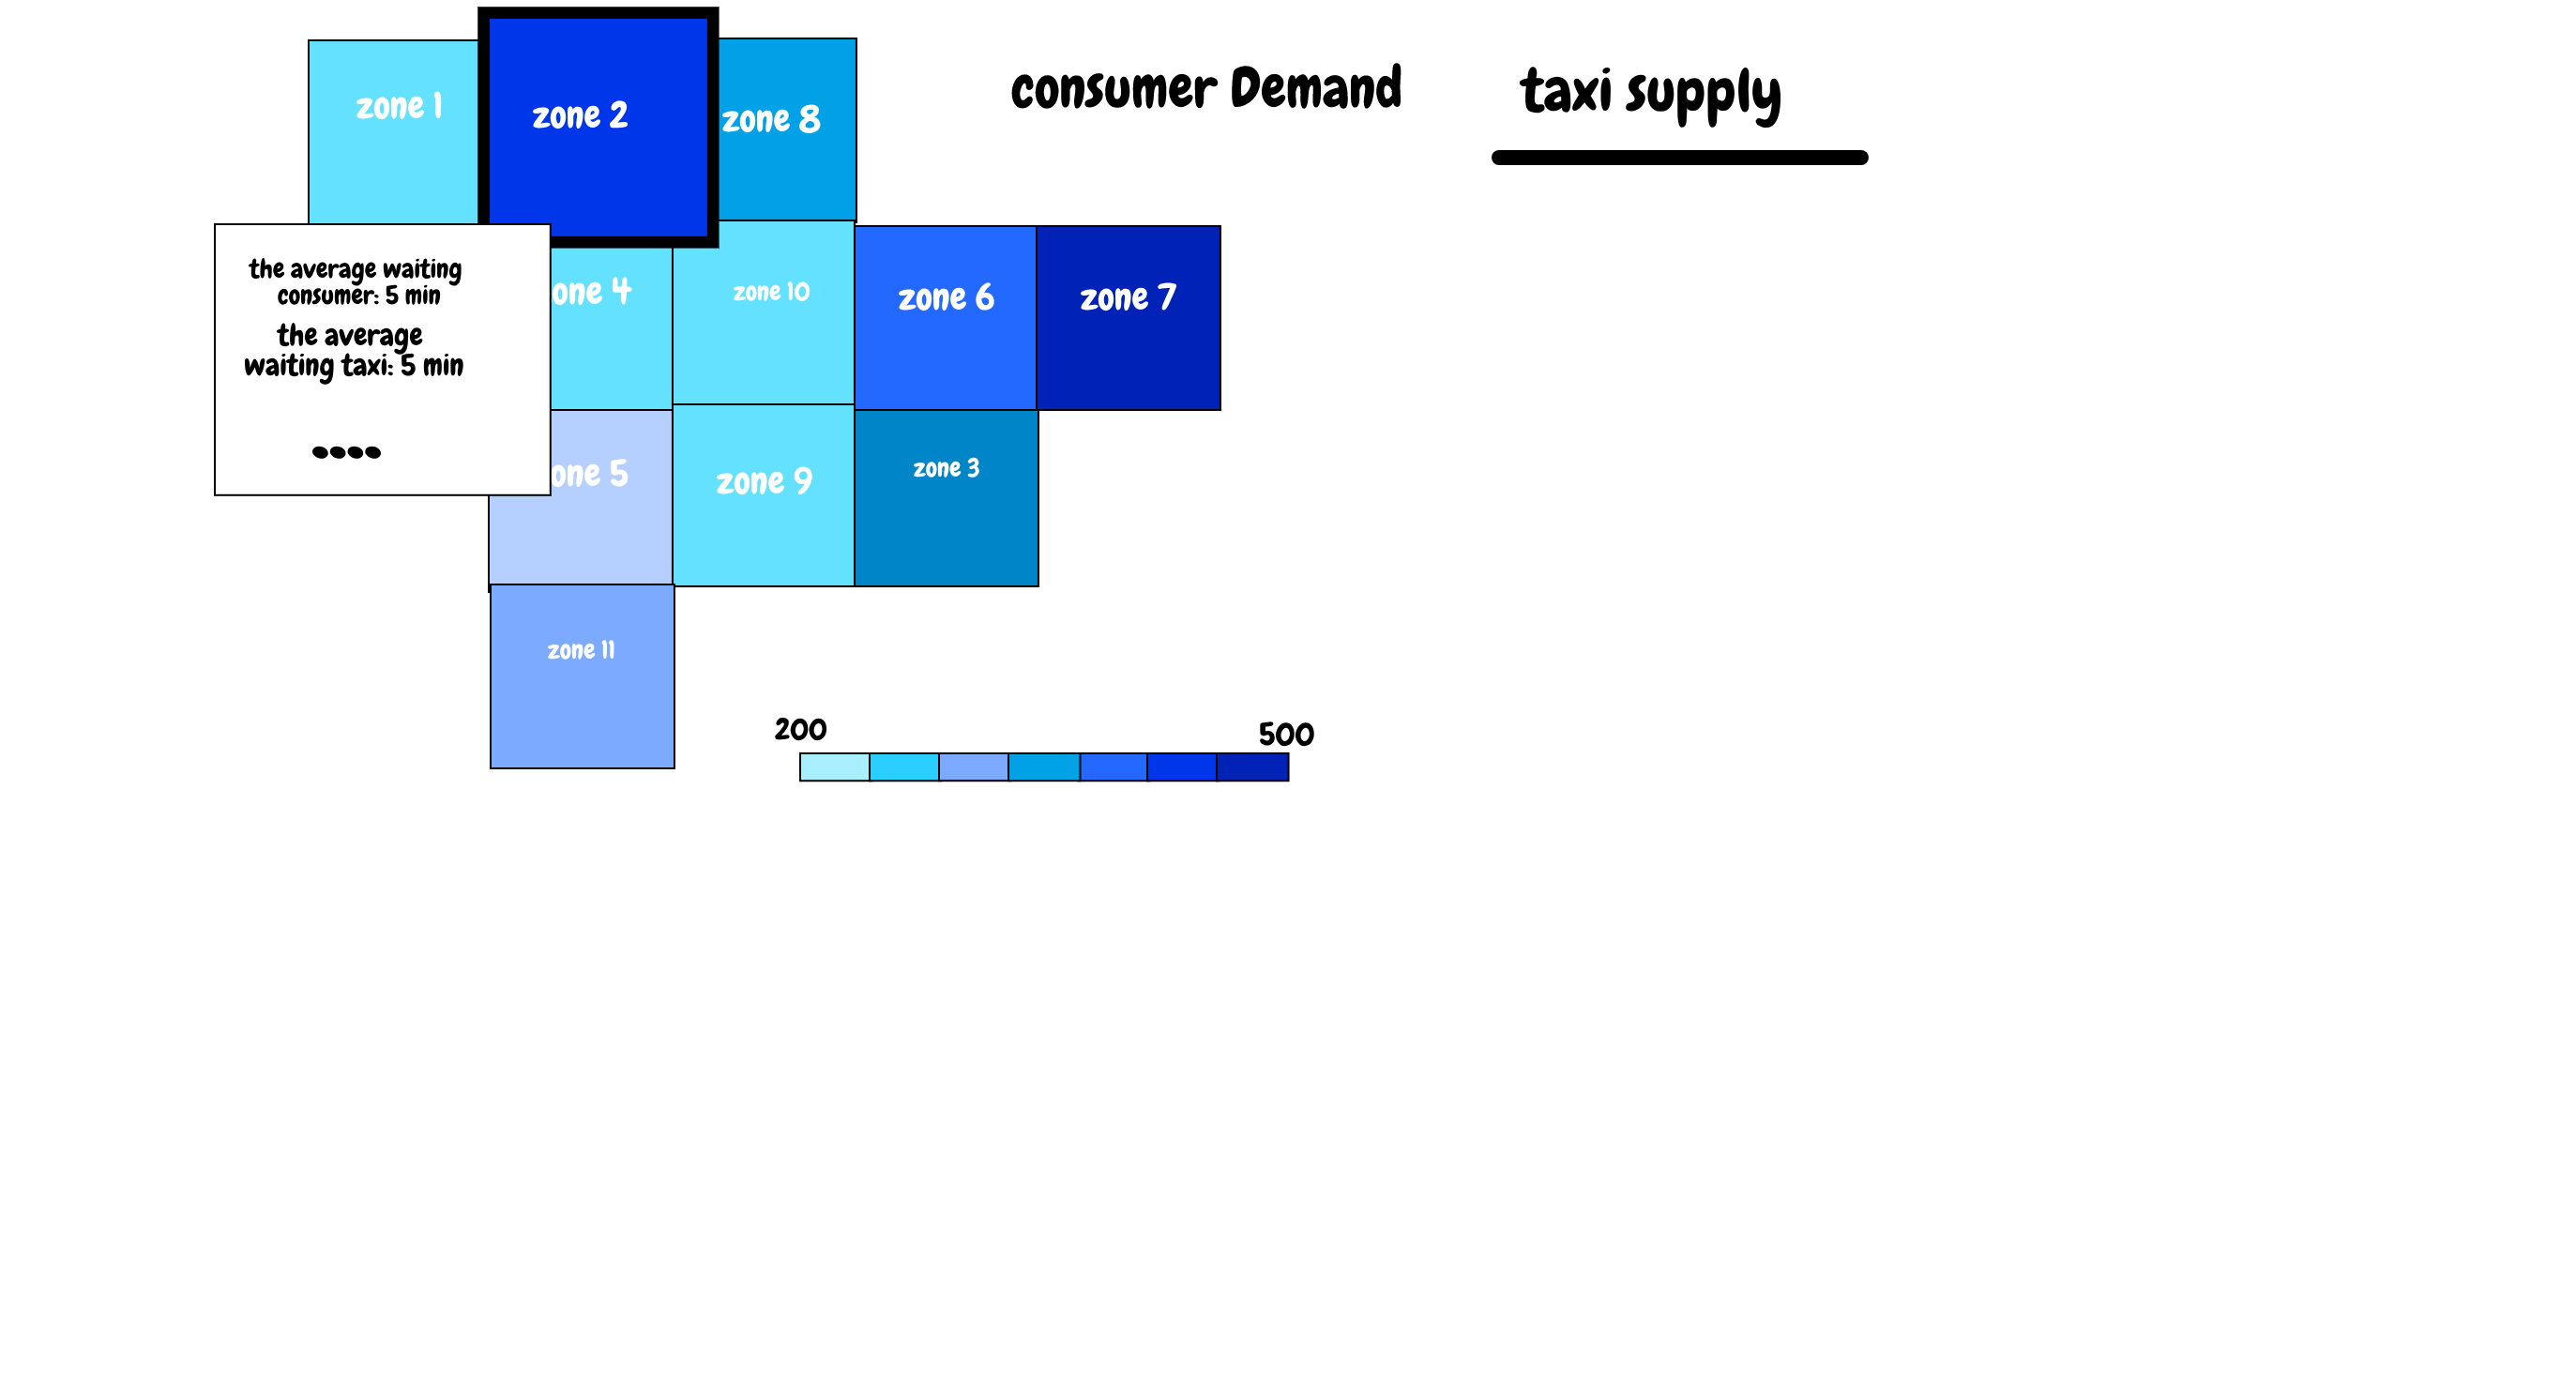
\includegraphics[width=0.8\textwidth]{sketch/stat_supply_tooltip.png}
                \caption{Tooltip}
              \end{figure}  

              \begin{figure}[h!]
                \centering
                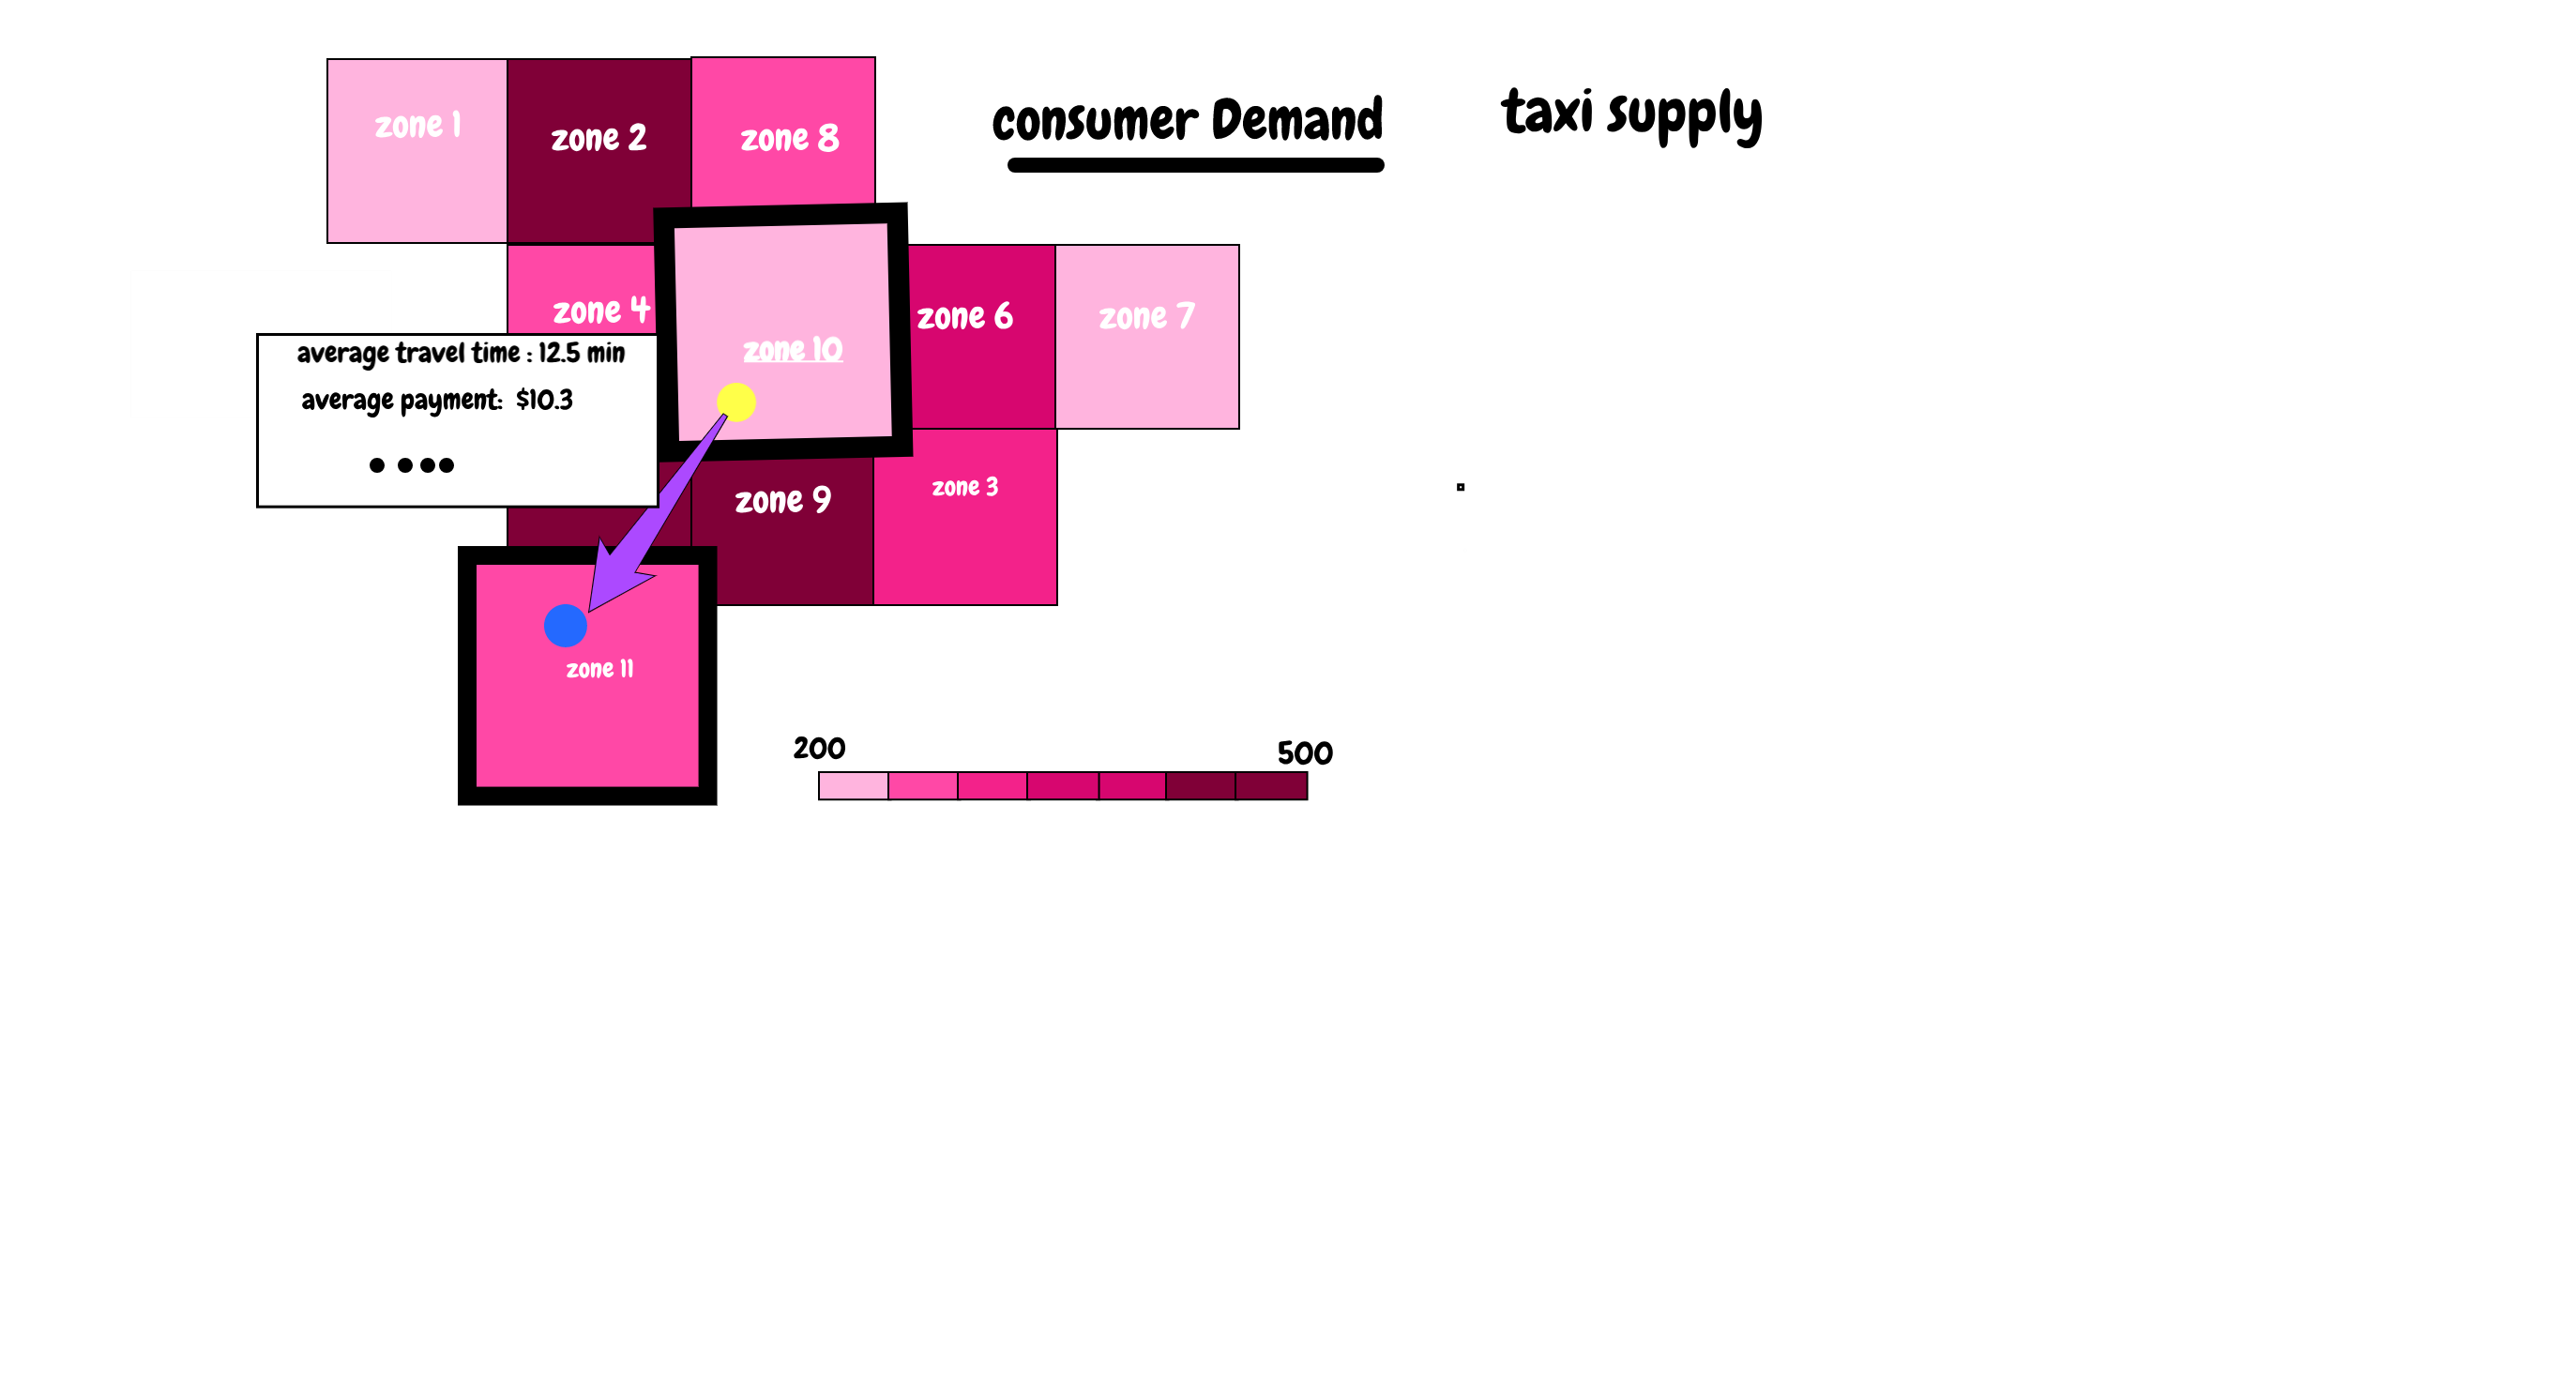
\includegraphics[width=0.8\textwidth]{sketch/stat_demand-tooltip.png}
                \caption{Zone Connection}
              \end{figure}  

        
            


\end{document}